% Doc preamble
\documentclass[11pt]{sig-alternate}
\usepackage{tabularx}
\usepackage{graphicx}
\usepackage{blindtext}
\usepackage[utf8]{inputenc}
\usepackage[english]{babel}
\usepackage{lastpage}
\usepackage{comment}
\usepackage{dirtytalk}
\usepackage{xcolor}
\usepackage{hanging}
\usepackage{wrapfig}
\usepackage[backend=biber, style=apa]{biblatex}
\addbibresource{notation.bib}
\usepackage{authblk}
\usepackage{caption}
\usepackage{longtable}
\usepackage{graphicx,subfigure}
\usepackage{authblk}
\usepackage{enumitem}
\usepackage[utf8]{inputenc}
\usepackage{cuted}
\usepackage{fancyhdr}
\usepackage{makecell}
\usepackage{xurl}
\usepackage{csquotes}
\usepackage{hyperref}
\usepackage{float}
\pagestyle{fancy}
\renewcommand{\headrulewidth}{0pt}
\renewcommand{\footrulewidth}{0pt}
\setlength\headheight{80.0pt}
\addtolength{\textheight}{-80.0pt}
\chead{%
  \ifcase\value{page}
  % empty test for page = 0
  \or 
\includegraphics[width=\textwidth]{headerImage.png}% page = 1
  \or 
\includegraphics[width=\textwidth]{headerImage.png}% page = 2
  \or 
\includegraphics[width=\textwidth]{headerImage.png}% page = 3
  \or 
\includegraphics[width=\textwidth]{headerImage.png}% page = 4
  \or 
\includegraphics[width=\textwidth]{headerImage.png}% page = 5
  \else
  
\includegraphics[width=\textwidth]{headerImage.png}
  \fi
}
%\chead{
\includegraphics[width=\textwidth]{headerImage.png}}
\fancyfoot[LE,LO]{Implementing Tactile Learning to Aid Students Understanding of the Bohr Model\\           
DOI: 10.14448/jsesd.14.0003}
\fancyfoot[CE,CO]{{ }}
\fancyfoot[RE,RO]{\thepage}
\pagenumbering{arabic}
\hypersetup{
    colorlinks=true,
    urlcolor=blue
}
 
\let\oldabstract\abstract
\let\oldendabstract\endabstract
\makeatletter
\renewenvironment{abstract}
{\renewenvironment{quotation}%
               {\list{}{\addtolength{\leftmargin}{1em} % change this value to add or remove length to the the default
                        \listparindent 1.5em%
                        \itemindent    \listparindent%
                        \rightmargin   \leftmargin%
                        \parsep        \z@ \@plus\p@}%
                \item\relax}%
               {\endlist}%
\oldabstract}
{\oldendabstract}
\makeatother
% end of preamble
\begin{document}


\title{Implementing Tactile Learning to Aid Students \\Understanding of the Bohr Model}
\begin{large}
\author[1]{\large \color{blue} Christin B. Monroe}
\author[1]{\large \color{blue} Andrew Stein}
\author[1]{\large \color{blue} Cynthia Tolman}

\affil[1]{Landmark College}
\end{large}
\toappear{}

\maketitle
\begin{@twocolumnfalse} 

\begin{abstract}
    \begin{large}
     \textit{It is essential for introductory level chemistry students to understand atomic models and how atoms interact to form chemical bonds. The tactile model in this article utilizes marbles to represent subatomic particles, a cup to represent the nucleus and wooden rings to simulate the electron orbitals. These inexpensive items can be combined to construct models in which students can build foundational knowledge of atomic structure and how subatomic particles interact. Students were asked to provide feedback comparing the use of this tactile model to atomic computer simulations, videos and their textbook regarding the method they felt was most useful to learn atomic structure.}\\
    \end{large}
\end{abstract}
\end{@twocolumnfalse}

%% ABSTRACT


%% AUTHOR INFORMATION

\textbf{*Corresponding Author, Christin Monroe}\\
\href{mailto:christinmonroe@landmark.edu}{(christinmonroe@landmark.edu)} \\
\textit{Submitted March 15, 2022 }\\
\textit{Accepted April 20, 2022} \\
\textit{Published online July 15, 2022} \\
\textit{DOI: 10.14448/jsesd.14.0003} \\


\pagebreak
\pagebreak

\vspace{5mm}
\section*{\vspace{140mm}}
\section*{Background}
\begin{large}
\subsection*{\textit{Definition of Neurodiversity}}
Neurodiversity is a social ideal based on a biological fact. The human brain is the most complex thing on Earth, and every brain is different. Neurodiversity is about what that should mean. Instead of separating people into normal and abnormal, neurodiversity asks us to accept variation. To us, it means that autism, ADHD, and learning disabilities are valuable forms of humanity that enrich culture. New ideas, insights, and unique ways of viewing the world come from diverse minds. This is a strength. (Center for Neurodiversity, n.d.)

\subsection*{\textit{The Use of Models in Education}}
Chemistry students tend to struggle with the abstract nature of the atomic structure because these structures can only be seen with the most powerful electron microscopes.(Netzell, 2014) Instead, models can aid students with visualizing and manipulating challenging microscopic structures. Following the discoveries of JJ Thompson and Ernest Rutherford in the mid-19th and early 20th centuries, respectively, the Bohr atom was developed in 1913 by Niels Bohr.(Neth et al. 2018) There has been some controversy as to whether the Bohr atom should be introduced and emphasized in Chemistry curriculum (for both secondary and postsecondary students), due to the possible misconceptions that can result.(Netzell, 2014),(Georgios \& Georgios, 2009) Also, there is no agreement on a methodology to teach atomic structure.(Derman et al., 2019) 

However, the Bohr atom can be an effective visual teaching aid as long as: 1) it is sufficiently compared and contrasted with other models, particularly the Schrödinger model and 2) limitations and potential misconceptions are identified and explored prior to introducing of the model.(McKagan et al., 2008) The Bohr model can also be used to help students make predictions about chemical behaviors.(Derman et al., 2019) 

A tactile Bohr atom model, made of marbles and inexpensive wood, allows students to visualize atoms isotopes and ions as large as neo\-dymium with 60 electron divots within the same inclusive model. 

Likely due to the rise in popularity of computer-generated models, there are few physical model kits that can be used in the classroom to teach the Bohr model in a tactile way.(Smiar \& Mendez, 2016) One study shows how 3D printed models of the Bohr atom can be created.(Smiar \& Mendez, 2016) 3D printing can be time consuming and limited to one atom at a time. The model kit presented herein is similar to others utilizing household materials to represent various chemical concepts, such as the octet rule (Lin et al., 2018) and periodicity (in the periodic table)(Melaku et al., 2016). 

Demonstrated use of models can help students gain an understanding of how scientists practice their thought-processes. (McKagan et al., 2008) Models have also been shown to increase communication and boost student understanding of complex scientific concepts.(Harrison \& Treagust, 2000) The simplicity of this model and the way in which it gives students the ability to physically manipulate it themselves (with explicit instructions) can decrease cognitive load. Decreasing cognitive load can lead to enhanced learning, especially for students with learning differences. (Carlson et al., 2003) Students with language disabilities can also greatly benefit from the incorporation of visual and tactile models. (Hudson, 2017)

The model presented in this article shows a multimodal approach where students are able to use the Bohr atom to: 1) manipulate the model using tactile functionality, 2) demonstrate their understanding by drawing the models they have created and 3) engage in dialogue with the instructor and their peers.

\subsection*{\textit{Inspiration and Development}}
Cynthia Tolman, the developer of the hands-on Bohr model, was inspired to create this model to provide students with a three-dimensional tool. The idea for making the models three-dimensional rather than flat allows the lower energy levels to be physically lower, showing that excited electrons ``fall" to a lower energy level when they re-emit their excess energy as light.

The first model was made from Styrofoam which was cut by hand into rings with an exacto knife, shown in figure 1. The Styrofoam was messy to work with and took a long time to cut through with the tools available. A second attempt using cardboard was easier to make but too flimsy for classroom use, shown in figure 2. The final design uses a CNC milling machine with ``Easel" software from Inventables. The design can be cut in wood or plastic and multiple models can be cut fairly quickly. The base is three stair-step blocks upon which the rings are glued or screwed. A plastic cup fits into the center ring to represent the nucleus and as in the previous designs, colored marbles represent protons, neutrons and electrons.

\begin{figure}[t]
    \centering
    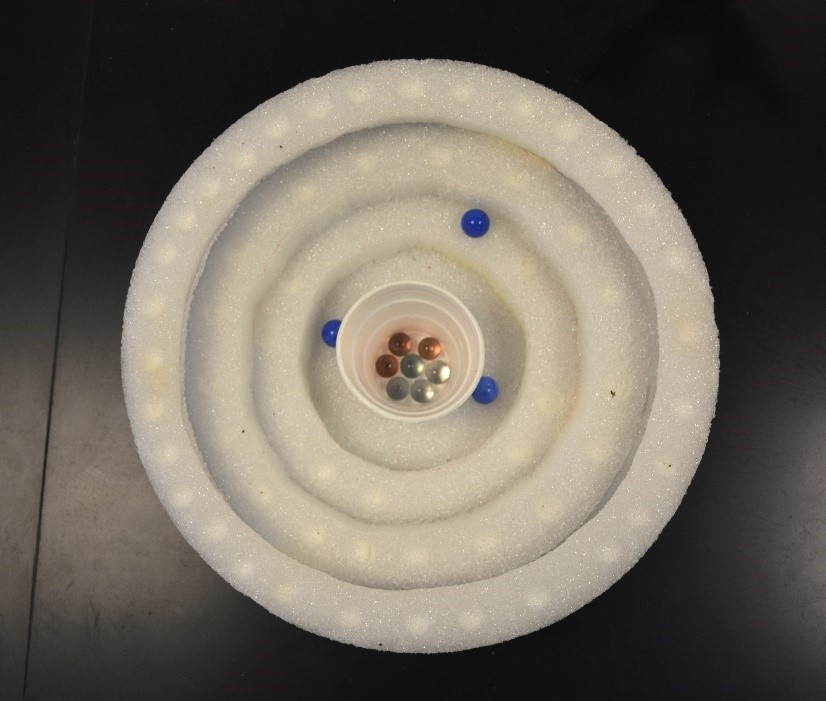
\includegraphics[width=\columnwidth]{figure 1_1.jpg}
\end{figure}

\begin{figure}[h!]
    \centering
    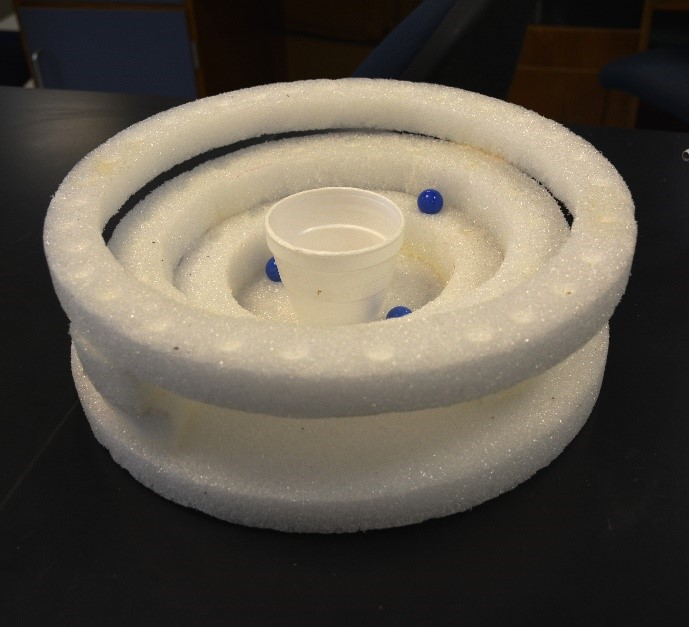
\includegraphics[width=\columnwidth]{figure 1_2.jpg}
    \captionsetup{font=large, labelfont=it}
    \caption{\textit{Second iteration of the hands-on Bohr model using Styrofoam and colored marbles.}}
    \label{Figure 1}
\end{figure}

\section*{Uses of the Model}
\subsection*{\textit{Representing Subatomic Particles }}
Having a general understanding of the structure of the atom is critical to understanding central chemical concepts. The proper placement and understanding of how subatomic particles (protons, neutrons, and electrons) are related to one another in the atomic model is essential to understanding how and why ions form and the mechanics involved in the formation of ionic compounds. The microscopic nature of subatomic particles prevents their direct observation which can be a challenging for students who thrive with visual and tactile learning.

In this model, each subatomic particle is represented by a different colored marble (protons: pink, electrons: blue and neutrons: clear). Students are initially instructed to build a hydrogen atom and a deuterium atom placing proton(s) and neutron(s) in the central cup representing the nucleus and electron(s) in the outer rings that surround the nucleus, as shown in Figure 3.

\begin{figure}[htp]
    \centering
    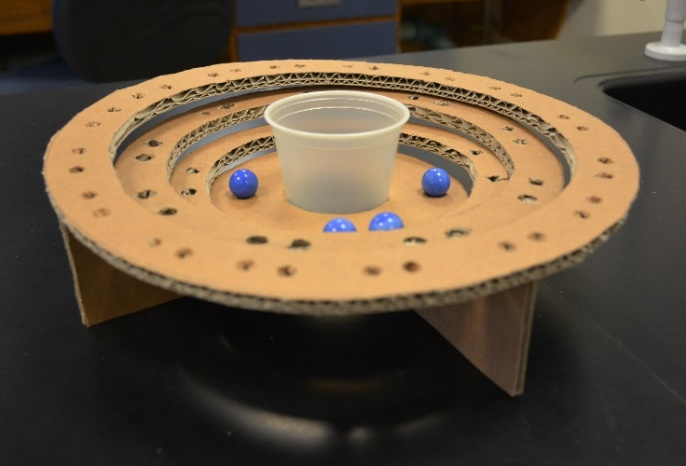
\includegraphics[width=\columnwidth]{figure 2.png}
    \captionsetup{font=large, labelfont=it}
    \caption{\textit{Third iteration of the hands-on Bohr model using cardboard and colored marbles.}}
    \label{Figure 2}
\end{figure}

\subsection*{\textit{Ions vs. Isotopes}}
Understanding how changing the numbers of different subatomic particles affects the identity of the element is often challenging for students, especially when differentiating between ions (modifying the number of electrons) and isotopes (modifying the number of neutrons). Students can be asked to change the number of protons, neutrons and electrons using this model. Changing the number of protons changes the identity of the atom, and keeping the protons in the nucleus (central cup) visually demonstrates that gain/ loss of protons is very unlikely. Changing the number of neutrons in the nucleus leads to the formation of a different isotope, but this is another process that does not commonly happen. Electrons, that surround the nucleus, are the easiest subatomic particle to add/ subtract and the removal/ addition of electrons is the only way to change the overall charge of the ion. If the total protons and electrons are not equal, the atom is either positively charged (cation) or negative charged (anion).

\begin{figure}[h!]
    \centering
    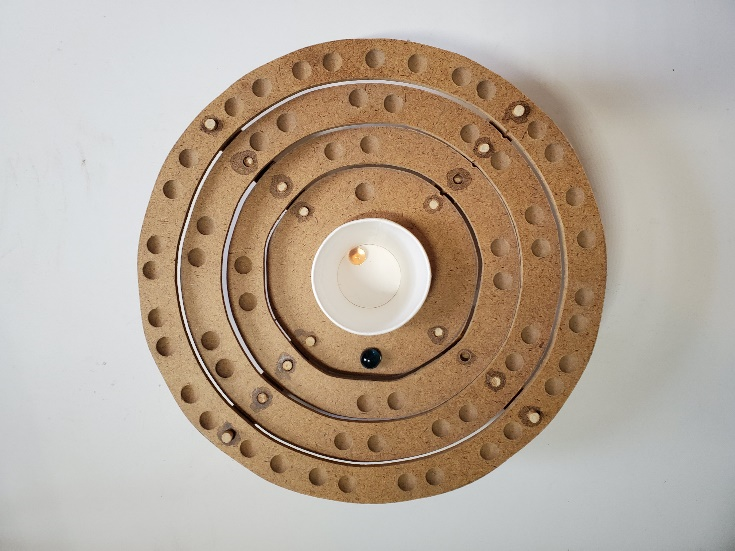
\includegraphics[width=\columnwidth]{figure 3_1.png}
\end{figure}
\begin{figure}[h!]
    \centering
    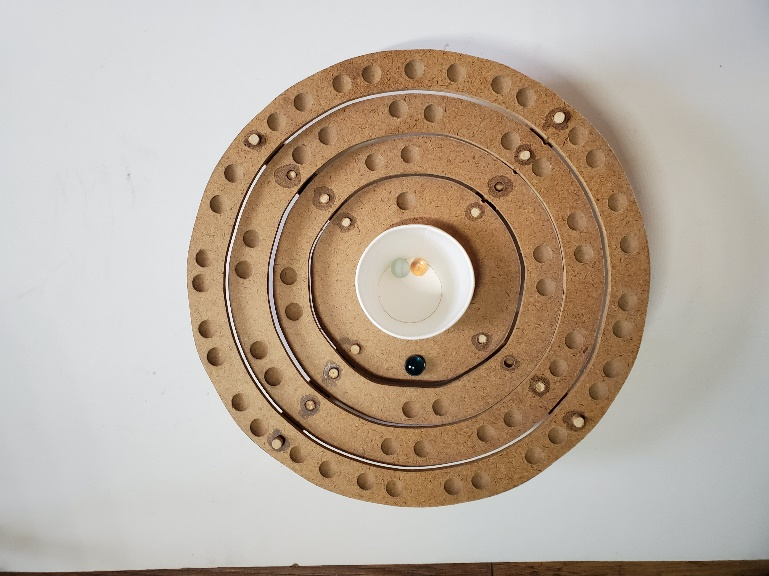
\includegraphics[width=\columnwidth]{figure 3_2.png}
    \captionsetup{font=large, labelfont=it}
    \caption{\textit{Two isotopes of hydrogen. Top: protium and Bottom: deuterium. Marbles represent subatomic particles. Blue represents electrons, pink represents protons and clear represents neutrons.}}
    \label{figure 3}
\end{figure}

\subsection*{\textit{Ion Formation Examples}}
Ions form to attain stable (electron) configurations by gaining or losing of electrons. After students are introduced to the concept of valance electrons and stable electron configurations, they can use the models to predict chemical behaviors. For example, the types of ions that would form to attain the most stable electron configuration. This model allows students to use visual cues to observe how electrons surround the nucleus.

Figure 4 shows a lithium atom in comparison to a lithium ion. When students observe the lithium atom, they work through the process of determining how best to achieve a stable electron configuration, either removal of 1 electron or addition of 7 electrons.

\begin{figure}[t!]
    \centering
    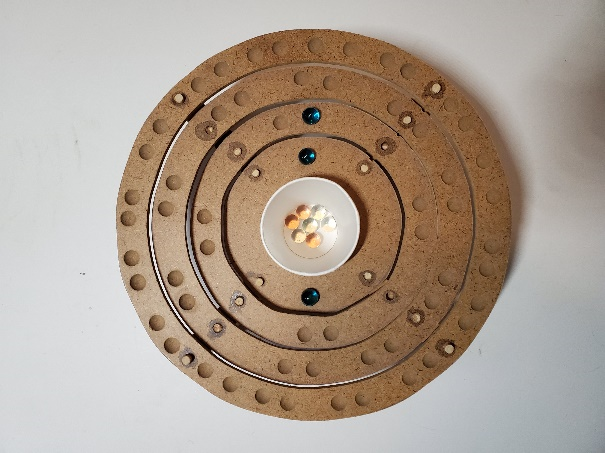
\includegraphics[width=\columnwidth]{figure 4_1.png}
    \captionsetup{font=large, labelfont=it}
    \caption{\textit{Comparison of a lithium atom (left) to a lithium ion (right).}}
    \label{Figure 4}
\end{figure}
\begin{figure}[t!]
    \centering
    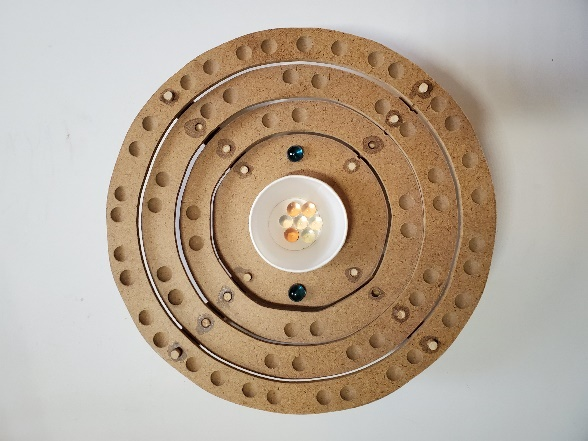
\includegraphics[width=\columnwidth]{figure 4_2.png}
\end{figure}

\subsection*{\textit{Quantization and Atomic Spectra}}
The concept of quantization (the idea that electrons can only absorb and emit certain energy levels and discrete energy levels) can first be introduced by showing the atomic spectra of various elements to students. Each element has a unique atomic spectrum, and each element has a unique distribution of electrons. In the Bohr model, there are specific locations where electrons can be located surrounding the nucleus, and this helps students grasp the quantization concept. In the model, there are divots on each energy level (circle surrounding the nucleus) that hold the electron marbles and represent the locations that electrons can occupy. The limitation of introducing quantization in this model is that all energy levels surrounding the nucleus are distributed evenly, but, the energy levels that surround the nucleus are not evenly distributed. This is a limitation that needs to be clearly stated as students are introduced to this concept. This can also be connected to atomic orbitals and the idea that no two electrons can occupy the same space. In this model, all energy levels are distributed evenly around the nucleus which is helpful conceptually but does not represent true electron distribution. This limits the introduction of quantization and requires an explicit explanation.

\subsection*{\textit{Excited vs.Ground States}}

The Bohr model can also be used to teach students to visualize the differences between an excited state vs. a ground state electron configuration. Students are first introduced to the idea that it takes energy to move negatively charge electrons away from the positively charged nucleus, because opposite charges attract. When enough energy is put into the system it will excite an electron, and it will move into a higher energy level (farther from the nucleus). As this concept is introduced it is again helpful to show students the atomic spectra of an element, so they can try to connect the unique spectra observed to the allowed excited states for a given element.

\begin{figure}[h!]
    \centering
    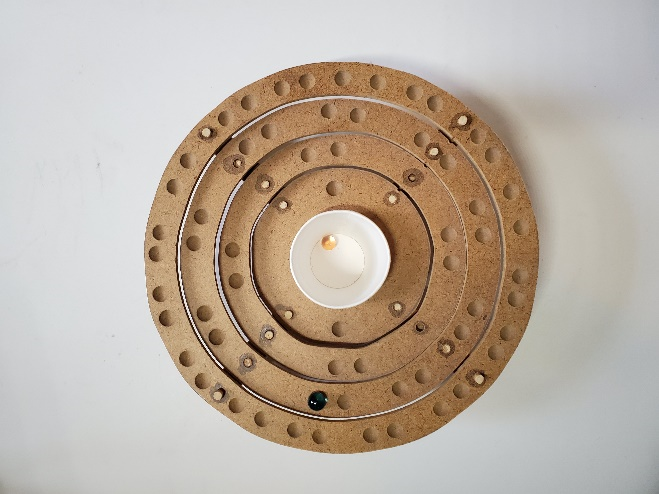
\includegraphics[width=\columnwidth]{figure 5.png}
    \captionsetup{font=large, labelfont=it}
    \caption{\textit{A hydrogen atom in an excited state.}}
    \label{Figure 5}
\end{figure}

\section*{Assessment of Student Learning}
This model has been used with both introductory biology and introductory chemistry students. Student learning was assessed by having students draw the Bohr models for at least three of the atoms they were asked to create. It has been shown that drawings are an effective way of determining students strengths and weaknesses in learning.(Gunstone, R. F., \& White, 2000) Students can also be provided with a pre-made drawing for them to fill in the proper placements of electrons.

To assess student understanding of prediction of chemical properties, students were asked to use the model to identify valance electrons and whether the ion donates or accepts electrons to form a stable electron configuration.

During these exercises, instructors are encouraged to circulate throughout the room to provide feedback to students as they place the marbles and fill in the written handout to represent the assigned atom.

\section*{Response from Students}
All procedures and materials were approved by a college IRB.

All students that were asked to participate in the Likert style survey (see Appendix) have been diagnosed as neurodiverse, as previously defined. Students were asked in class to complete a written survey. Of the 24 students in the class, 15 (63\% response rate) participated in the survey. The results of the 26 Likert scale sets of questions are summarized in Figure 6. Students found the hands-on model and computer simulations to be beneficial, with 74-77\% of respondents “strongly agreeing” or “agreeing” that the resources were helpful. Only 60\% of respondents found reading assignments helpful. By a large margin, more students (30\%) strongly agreed that the hands-on model was useful, compared to 15\% for computer simulations and 14\% for reading assignments. 87\% of respondents either agreed or strongly agreed that having access to all three resources would be their choice. 100\% of respondents agreed or strongly agreed that the hands-on Bohr model helped them understand atomic structure.

\begin{figure*}[t]
    \centering
    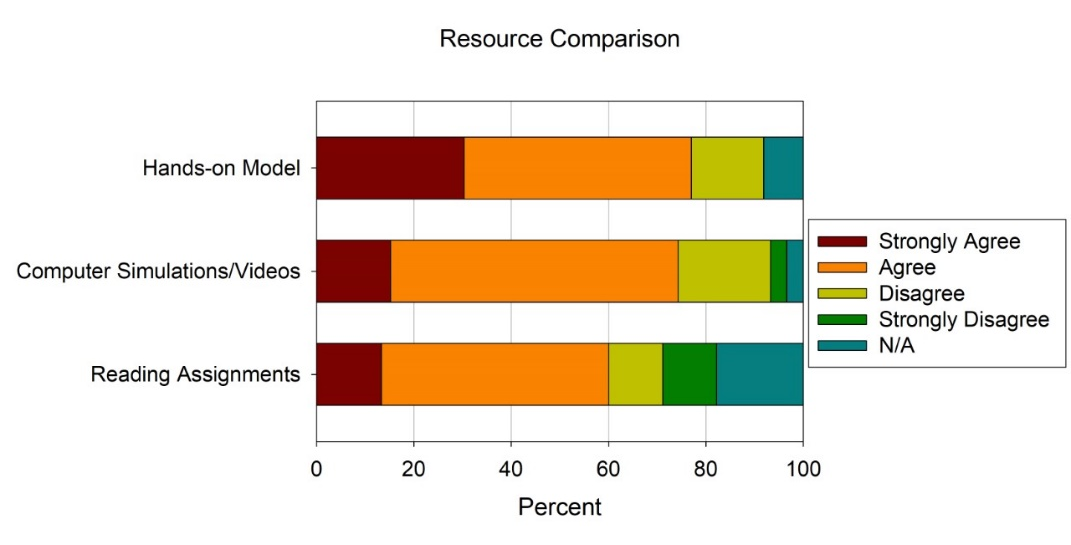
\includegraphics[width=\textwidth]{figure 6_1 crop.png}
\end{figure*}
\begin{figure*}[h!]
    \centering
    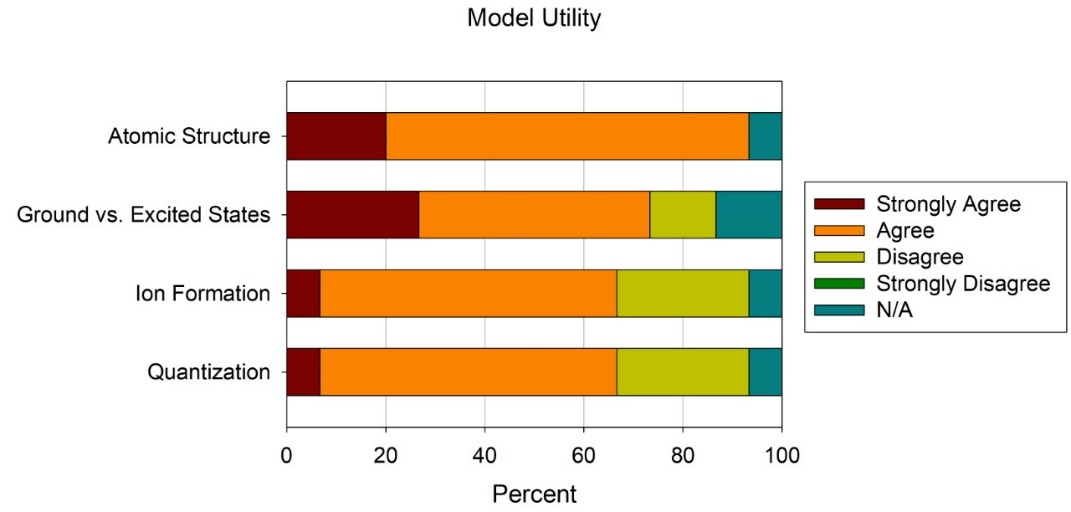
\includegraphics[width=\textwidth]{figure 6_2.png}
    \captionsetup{font=large, labelfont=it}
    \caption{\textit{Responses to survey questions given as the fraction of respondents selecting each Likert scale rating (participation count n=15). The top graph represents a summary of student responses assessing the usefulness of each teaching method to their learning style. The bottom graph represents responses to assess the usefulness of the hands-on Bohr model for each of the listed categories.}}
    \label{Figure 6}
\end{figure*}

\begin{figure}[h]
    \centering
    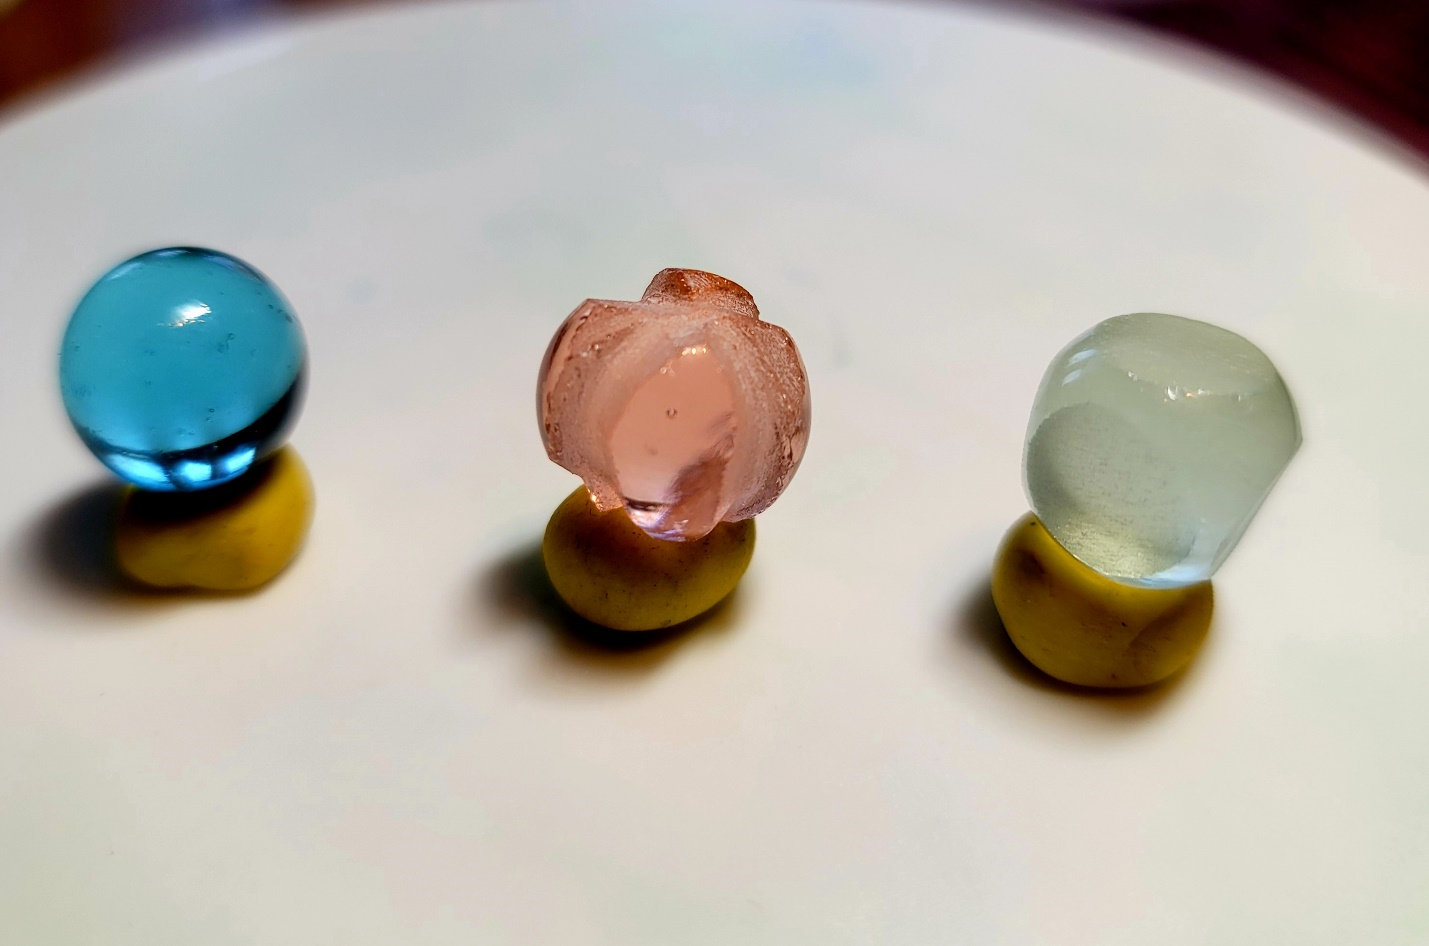
\includegraphics[width=\columnwidth]{figure 7.png}
    \captionsetup{font=large, labelfont=it}
    \caption{\textit{Etch patterns for proton (middle; represented by pink marbles that have single or double perpendicular etching around the center of the marble) and neutrons (right; represented by colorless marbles with circular flat edges on each side of the marble). Electrons (left; represented blue non-etched marble).}}
    \label{Figure 7}
\end{figure}
\section*{Future Directions}
The Bohr atomic model discussed in this paper was presented at the 2015 Annual Flipped Learning and the 2021 Inclusion in Science Learning in a New Direction (ISLAND) conferences, where it received positive feedback and comments. Some of the feedback related to expanding the sensory experience for students utilizing the Bohr model. Currently, ideas of etching the marbles are being considered to incorporate the sense of touch into the learning experience. This would also allow for students with visual impairments to benefit from the model. 

Figure 7 shows some initial ideas of how the marbles would be modified. Blue marbles, which depict electrons, would remain unchanged, for two reasons: 1) the marbles representing the electrons must be able to fit into the grooves of the atomic structure and 2) electrons are typically depicted as spheres or circles in textbooks, so the goal is to be as consistent as possible with traditional textbook depictions.

Pink marbles (representing protons) could be etched through the center of the marble, or have two perpendicular rings that are etched into the marble, as depicted in figure 7a. The perpendicular etches resemble a “plus sign”, which would make it easy for students to associate the crossed-etched marbles with protons. Colorless marbles (representing neutrons) could have two or four sides etched, show in figure 7b. Each side would have a circular flat edge, resembling a zero. The circular flat edge would help students associate the marbles with the neutral (net zero) charge of neutrons.

\section*{Conclusions}
This article demonstrates that a tactile and manipulatable Bohr atom model can aid students with of visualizing microscopic subatomic particles. This model can be used with students of diverse learning styles to understand a variety of concepts including: 1) subatomic particle placement in the atom, 2) distinguishing between ions and isotopes, 3) relating quantization to atomic spectra and 4) distinguishing between ground and excited states of atoms and ions. Overall, the student surveyed felt they learned best using either computational models or the hands-on model to reading assignments. Based upon the data, using a universal model, where students are exposed to multiple methods for teaching the Bohr model appears to be the most beneficial, based upon student feedback.

\section*{Acknowledgements}
The authors would like to thank Dr. Brian Young and Dr. Kim Coleman for their guidance and feedback on this project. The authors also thank Jennifer Lann for her research assistance for this project.

This material is based upon work supported by the National Science Foundation under Grant No 1643326 and 2129912.

\clearpage

\section*{References}\par 

\leftskip 0.25in
\parindent -0.25in 
%%%
Carlson, R., Chandler, P., \& Sweller, J. (2003). Learning and Understanding Science Instructional Material. \textit{Journal of Educational Psychology, 95}(3), 629–640. \url{https://doi.org/10.1037/0022-0663.95.3.629}

Center for Neurodiversity. (n.d.). \url{https://www.landmark.edu/center-for-neurodiversity}

Derman, A., Koçak, N., \& Eilks, I. (2019). Insights into components of prospective science teachers’ mental models and their preferred visual representations of atoms. \textit{Education Sciences, 9}(2), 1–19. \url{https://doi.org/10.3390/educsci9020154}

Neth, E. J., Flowers, P., Theopold, K., Langley, R., \& Robinson, W. R. (2018). Chemistry: Atoms First (OpenStax).

Georgios, T., \& Georgios, P. (2009). High-school students’ conceptual difficulties and attempts at conceptual change: the case of basic quantum concepts. \textit{International Journal of Science Education, 31}(7), 895–930.

Gunstone, R. F., \& White, R. (2000). Goals, methods and achievements of research in science education. In \textit{In Improving Science Education: The Contribution of Research} (pp. 293–307).

Harrison, A. G., \& Treagust, D. F. (2000). A typology of school science models. \textit{International Journal of Science Education, 22}(9), 1011–1026. \url{https://doi.org/10.1080/095006900416884}

Hudson, D. (2017). How to support dyslexic students. \textit{Education in Chemistry.} \url{https://edu.rsc.org/ideas/learning-difficulties-and-chemistry/3008085.article}

Lin, H. J., Lehoang, J., Kwan, I., Baghaee, A., Ha-chen, S. J., Moss, T., \& Woods, J. D. (2018). \textit{Article Lego Bricks and the Octet Rule: Molecular Models for Biochemical Pathways with Plastic, Interlocking Toy Bricks}. August 2017, 54–57. \url{https://doi.org/10.1002/bmb.21090}

McKagan, S. B., Perkins, K. K., \& Wieman, C. E. (2008). Why we should teach the Bohr model and how to teach it effectively. \textit{Physical Review Special Topics - Physics Education Research, 4}(1), 1–10. \url{https://doi.org/10.1103/PhysRevSTPER.4.010103}

Melaku, S., Schreck, J. O., Griffin, K., \& Dabke, R. B. (2016). Interlocking Toy Building Blocks as Hands-On Learning Modules for Blind and Visually Impaired Chemistry Students. \textit{Journal of Chemical Education, 93}(6), 1049–1055. \url{https://doi.org/10.1021/acs.jchemed.5b00252}

Netzell, E. (2014). \textit{Using models and representations in learning and teaching about the atom}. 1–74. \url{http://www.diva-portal.org/smash/get/diva2:807576/FULLTEXT01.pdf}

Smiar, K., \& Mendez, J. D. (2016). Creating and Using Interactive, 3D-Printed Models to Improve Student Comprehension of the Bohr Model of the Atom, Bond Polarity, and Hybridization. \textit{Journal of Chemical Education, 93}(9), 1591–1594. \url{https://doi.org/10.1021/acs.jchemed.6b00297}

\newpage

\section*{Supplementary Information}
\subsection*{\textit{CNC Patterns}}

Material type: Two-Color HDPE\\
Material dimensions: 12 in x 12 in x 0.25 in\\
Bit: 0.125 in, Straight cut\\
    \begin{figure}[htp]
        \centering
        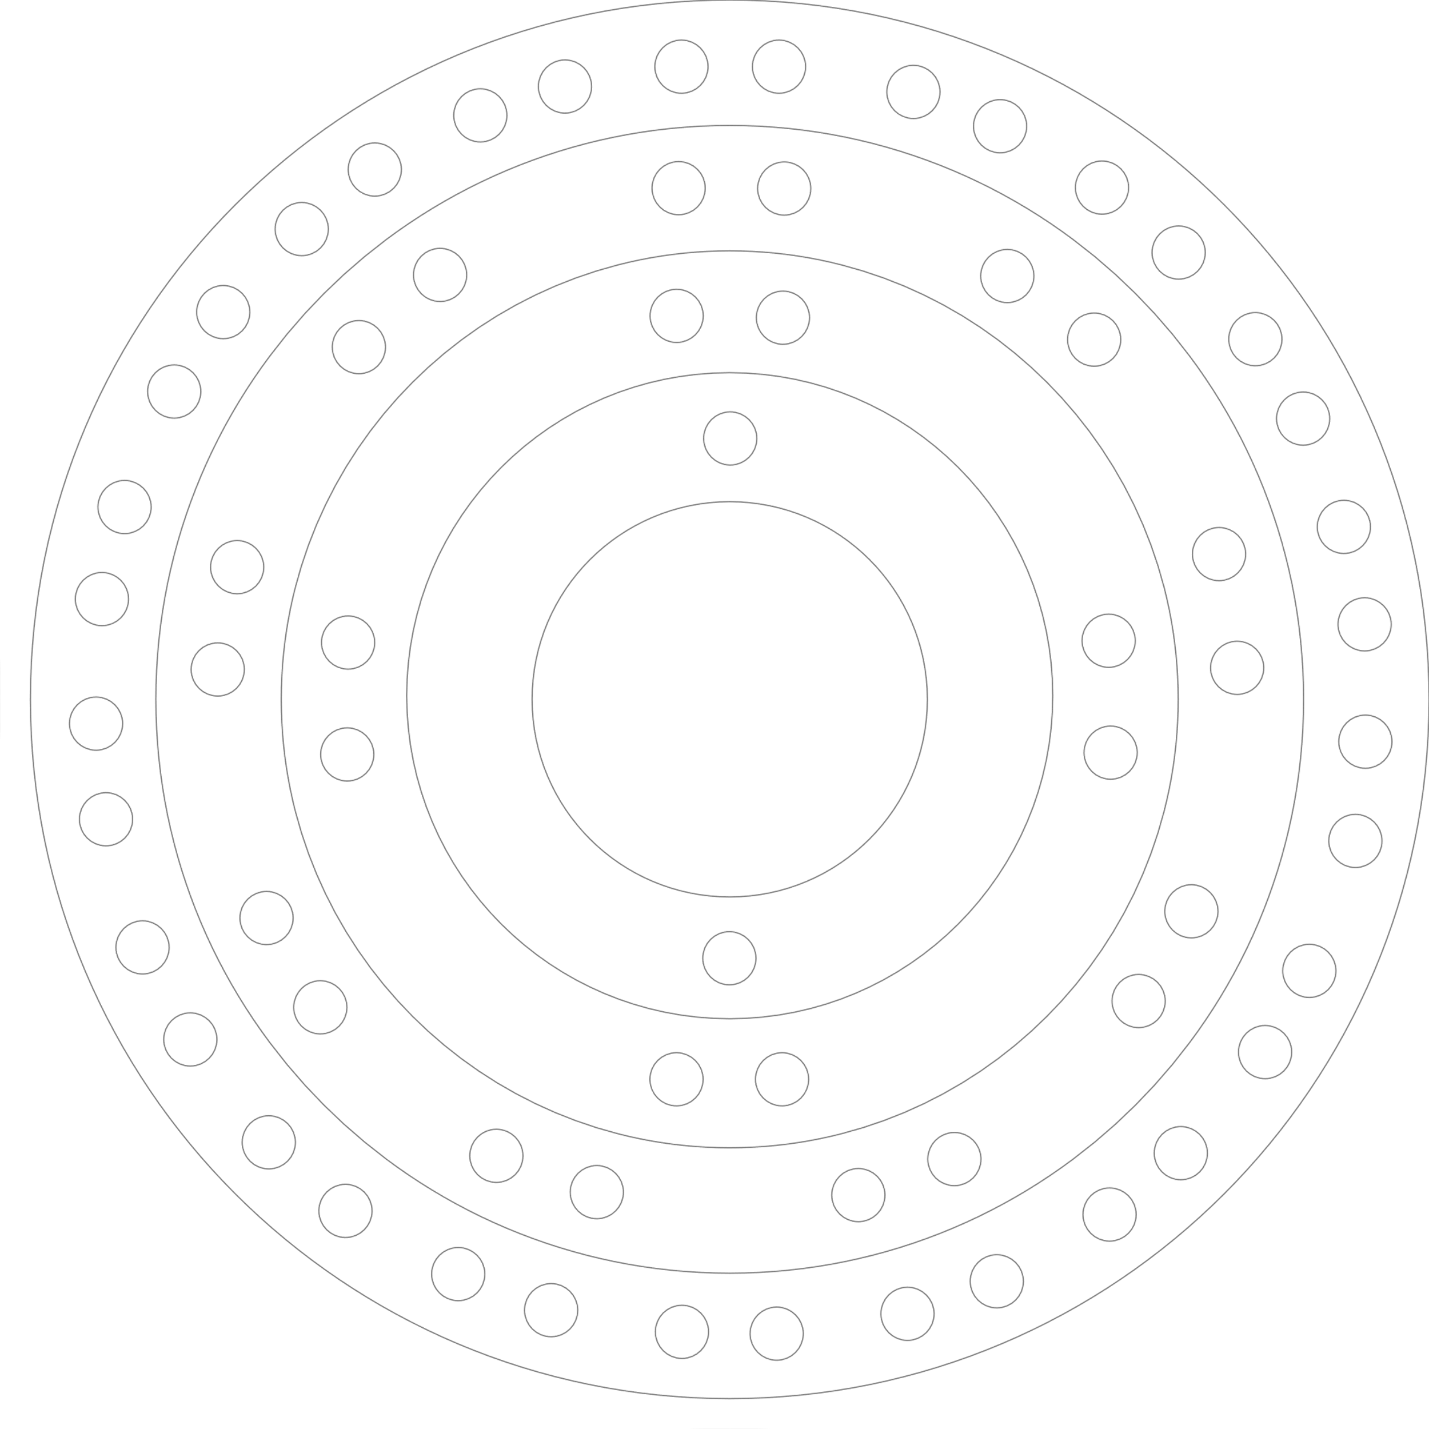
\includegraphics[width=15.5cm]{CNC pattern 1.png}
        \label{Image shows a blueprint for creating the 3D Bohr models.}
    \end{figure}

\clearpage
Material type: One-Color HDPE\\
Material dimensions: 24 in x 12 in x 0.5 in\\
Bit: 0.125 in, Straight cut
    \begin{figure}[h]
        \centering
        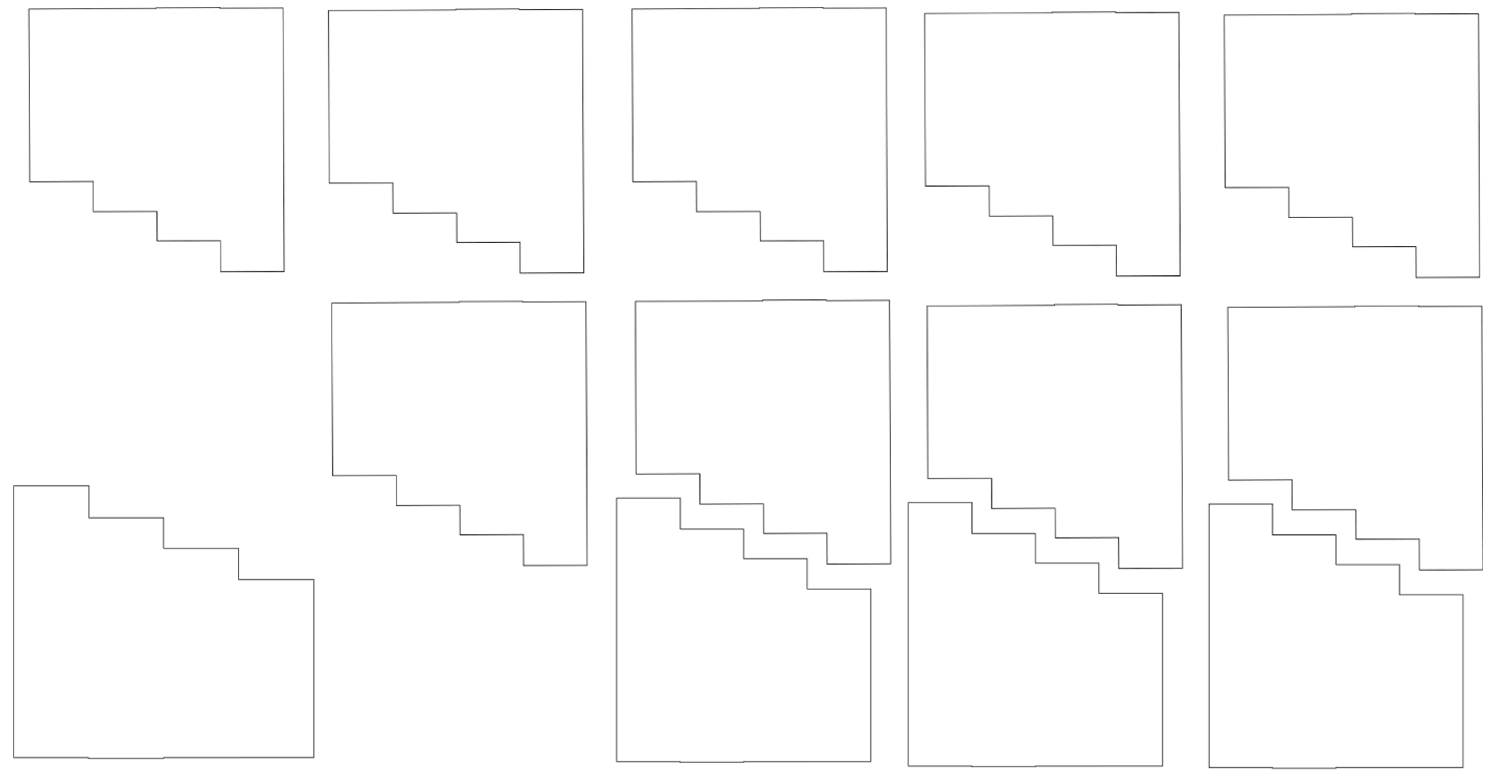
\includegraphics[width=\textwidth]{CNC pattern 2.png}
        \label{Image show a blue print with sizing/dimensions of the fabricated Bohr model.}
    \end{figure}

\clearpage 

Material type: One-Color HDPE\\
Material dimensions: 24 in x 12 in x 0.5 in\\
Bit: 0.125 in, Straight cut\\
    \begin{figure}[htp]
        \centering
        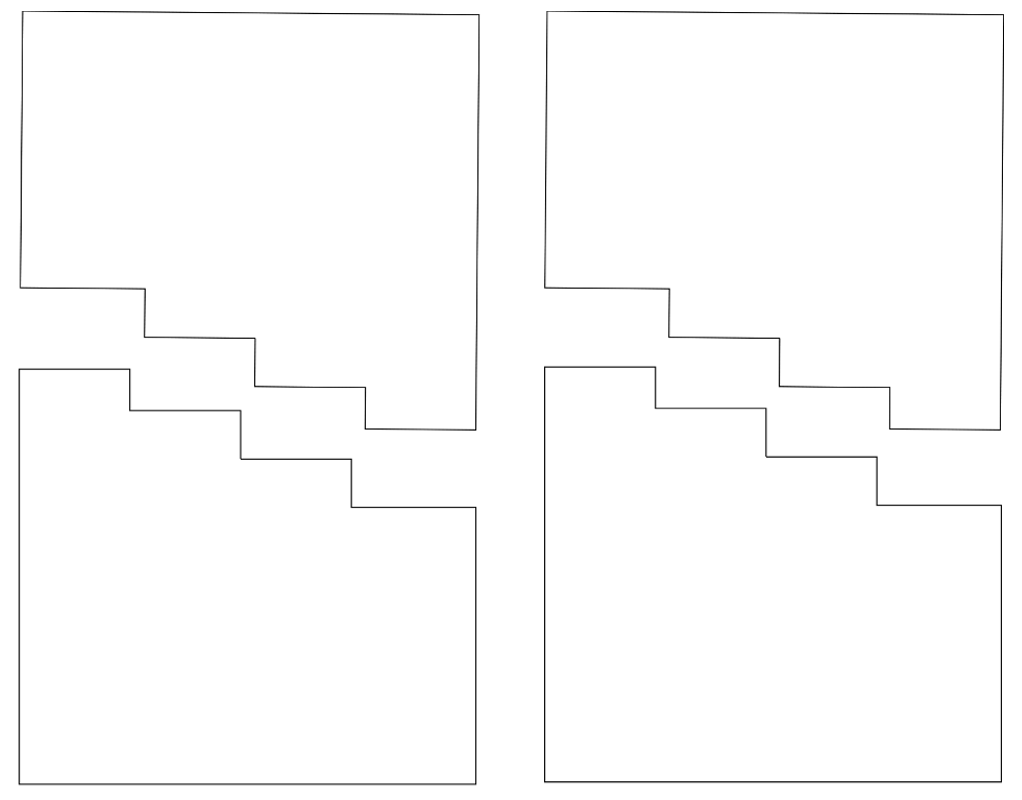
\includegraphics[width=\textwidth]{CNC pattern 3.png}
        \label{Image show a blueprint with sizing/dimensions of the fabricated Bohr model.}
    \end{figure}
    
\clearpage

\onecolumn
\leftskip 0 in
\parindent -0 in 

\subsection*{\textit{Student Consent Form}}
\subsubsection*{Consent Form}

\subsubsection*{\textbf{DESCRIPTION OF STUDY}}
My name is Dr. Christin Monroe and I am a Visiting Assistant Professor of Chemistry at Landmark College. I am conducting a study with the purpose of comparing the use of tactile learning techniques vs. computer simulations for learning about atomic structure. I am asking for your voluntary consent to complete a single survey that should last no longer than 15 minutes. The goal of this study is to understand which techniques are more meaningful for students learning about atomic structure, not to evaluate your abilities.

\subsubsection*{\textbf{SURVEY}}
If you agree to participate, after the completion of the atomic structure component of Introduction to Chemistry or Principles of Chemistry I/II you will be asked to take a short survey that will last no longer than 15 minutes that will ask you to compare computer simulations about atomic structure to the hands-on Bohr model. All surveys will be submitted anonymously. You will only be asked to compare the two types of learning with your own learning style.

\subsubsection*{\textbf{RISKS}}
There are no known risks to participating in this study.

\subsubsection*{\textbf{BENEFITS}}
Your feedback will contribute to the academic conversation regarding how the atom is taught in the undergraduate chemistry classroom. If you are interested, you will be provided access to the final report once this study has been completed and documented. 

\subsubsection*{\textbf{CONFIDENTIALITY}}
All data collected in this study will remain confidential, and all person-identifiable data (e.g. IP address tracking) will disabled so you cannot be personally identified. Data from this study will be kept in a password protected account in SurveyMonkey or in a locked file cabinet in a locked room until it is destroyed. Data will not be retained for more than 5 years.

\subsubsection*{\textbf{PARTICIPATION}}
Your participation is voluntary, and you may withdraw from the study for any reason at any time. There is no penalty for withdrawing from the study or choosing not to participate. 

\subsubsection*{\textbf{CONTACT}}
This study is being conducted by the History Department at Landmark College. The lead evaluator is Dr. Christin Monroe, who can be reached by calling 802.387.1640, or by email at \href{mailto:csupalo@ets.org}{(christinmonroe@landmark.edu)}. 

If you have questions about the research process or your rights as a human subject, please contact Dr. Adam Lalor, Chair, Institutional Review Board of Landmark College, at 802-387-6735 or \url{https://intranet.landmark.edu/research-office/irb.cfm.}

\subsubsection*{\textbf{CONSENT}}
I have read this form and indicate my decision to participate or not participate as follows:\\

I am 18 years old or over\\

I \textbf{agree} to participate in this study.\\

I \textbf{do not agree} to participate in this study.\\

Signature:\\

Date:\\

Print name:\\

\clearpage

\subsection*{\textit{Likert Student Questionnaire}}
\begin{table}[]
\resizebox{\textwidth}{!}{%
\begin{tabular}{ll|c|c|c|c|c|}
\cline{3-7}
 &
   &
  \begin{tabular}[c]{@{}c@{}}Strongly \\ Agree\end{tabular} &
  Agree &
  Disagree &
  \begin{tabular}[c]{@{}c@{}}Strongly \\ Disagree\end{tabular} &
  \begin{tabular}[c]{@{}c@{}}Neither \\ or N/A\end{tabular} \\ \hline
\multicolumn{1}{|l|}{1.} &
  \begin{tabular}[c]{@{}l@{}}I find it easy to visualize microscopic \\ concepts (i.e., cells, atoms, chemical \\ reactions) when using text and computer \\ simulations.\end{tabular} &
  4 &
  3 &
  2 &
  1 &
  0 \\ \hline
\multicolumn{1}{|l|}{2.} &
  \begin{tabular}[c]{@{}l@{}}After reading the textbook, I felt I had \\ a strong understanding of atomic structure.\end{tabular} &
  4 &
  3 &
  2 &
  1 &
  0 \\ \hline
\multicolumn{1}{|l|}{3.} &
  \begin{tabular}[c]{@{}l@{}}I find computer simulations make it easier \\ to understand microscopic concepts.\end{tabular} &
  4 &
  3 &
  2 &
  1 &
  0 \\ \hline
\multicolumn{1}{|l|}{4.} &
  \begin{tabular}[c]{@{}l@{}}If given a choice, I would prefer to use \\ hands on activities to learn about \\ microscopic concepts.\end{tabular} &
  4 &
  3 &
  2 &
  1 &
  0 \\ \hline
\multicolumn{1}{|l|}{5.} &
  \begin{tabular}[c]{@{}l@{}}I do not feel that I can fully understand \\ a microscopic concept unless the \\ lesson involves a model that involves \\ tactile learning techniques.\end{tabular} &
  4 &
  3 &
  2 &
  1 &
  0 \\ \hline
\multicolumn{1}{|l|}{6.} &
  \begin{tabular}[c]{@{}l@{}}If given a choice, I would prefer to use \\ computer simulations to learn about \\ microscopic concepts.\end{tabular} &
  4 &
  3 &
  2 &
  1 &
  0 \\ \hline
\multicolumn{1}{|l|}{7.} &
  \begin{tabular}[c]{@{}l@{}}After watching videos I felt I had a strong \\ understanding of atomic structure.\end{tabular} &
  4 &
  3 &
  2 &
  1 &
  0 \\ \hline
\multicolumn{1}{|l|}{8.} &
  \begin{tabular}[c]{@{}l@{}}I find that hands-on activities make it \\ easier to understand microscopic concepts.\end{tabular} &
  4 &
  3 &
  2 &
  1 &
  0 \\ \hline
\multicolumn{1}{|l|}{9.} &
  \begin{tabular}[c]{@{}l@{}}If given a choice, I would prefer to use \\ all three (text, hands-on activities and \\ computer simulations to learn) about \\ microscopic concepts.\end{tabular} &
  4 &
  3 &
  2 &
  1 &
  0 \\ \hline
\multicolumn{1}{|l|}{10.} &
  \begin{tabular}[c]{@{}l@{}}Before using the computer simulation I \\ understood atomic structure.\end{tabular} &
  4 &
  3 &
  2 &
  1 &
  0 \\ \hline
\multicolumn{1}{|l|}{11.} &
  \begin{tabular}[c]{@{}l@{}}After using the computer simulation I \\ understood atomic structure.\end{tabular} &
  4 &
  3 &
  2 &
  1 &
  0 \\ \hline
\multicolumn{1}{|l|}{12.} &
  \begin{tabular}[c]{@{}l@{}}Before using the hands-on Bohr model I \\ understood atomic structure.\end{tabular} &
  4 &
  3 &
  2 &
  1 &
  0 \\ \hline
\multicolumn{1}{|l|}{13.} &
  \begin{tabular}[c]{@{}l@{}}After using the hands-on Bohr model I \\ understood atomic structure.\end{tabular} &
  4 &
  3 &
  2 &
  1 &
  0 \\ \hline
\multicolumn{1}{|l|}{14.} &
  \begin{tabular}[c]{@{}l@{}}The computer simulation helped me to \\ understand how ions form.\end{tabular} &
  4 &
  3 &
  2 &
  1 &
  0 \\ \hline
\multicolumn{1}{|l|}{15.} &
  \begin{tabular}[c]{@{}l@{}}The hands-on Bohr model helped me to \\ understand how ions form.\end{tabular} &
  4 &
  3 &
  2 &
  1 &
  0 \\ \hline
\multicolumn{1}{|l|}{16.} &
  \begin{tabular}[c]{@{}l@{}}Before using the hands-on Bohr model I \\ understood how subatomic particles \\ (protons, neutrons, electrons) were placed \\ around the nucleus.\end{tabular} &
  4 &
  3 &
  2 &
  1 &
  0 \\ \hline
\multicolumn{1}{|l|}{17.} &
  \begin{tabular}[c]{@{}l@{}}I learn best when a variety of techniques \\ are combined to teach microscopic \\ concepts.\end{tabular} &
  4 &
  3 &
  2 &
  1 &
  0 \\ \hline
\multicolumn{1}{|l|}{18.} &
  \begin{tabular}[c]{@{}l@{}}Before using the hands-on Bohr model I \\ understood the concept of quantization.\end{tabular} &
  4 &
  3 &
  2 &
  1 &
  0 \\ \hline
\multicolumn{1}{|l|}{19.} &
  \begin{tabular}[c]{@{}l@{}}I find I learn best when working with \\ models using my hands.\end{tabular} &
  4 &
  3 &
  2 &
  1 &
  0 \\ \hline
\multicolumn{1}{|l|}{20.} &
  \begin{tabular}[c]{@{}l@{}}After using the hands-on Bohr model I \\ understood the concept of quantization.\end{tabular} &
  4 &
  3 &
  2 &
  1 &
  0 \\ \hline
\multicolumn{1}{|l|}{21.} &
  I find I learn best when watching videos. &
  4 &
  3 &
  2 &
  1 &
  0 \\ \hline
\multicolumn{1}{|l|}{22.} &
  \begin{tabular}[c]{@{}l@{}}Using the hands-on Bohr model helped \\ me to understand the difference between \\ ground and excited states.\end{tabular} &
  4 &
  3 &
  2 &
  1 &
  0 \\ \hline
\multicolumn{1}{|l|}{23.} &
  \begin{tabular}[c]{@{}l@{}}I find I learn best when reading the \\ textbook.\end{tabular} &
  4 &
  3 &
  2 &
  1 &
  0 \\ \hline
\multicolumn{1}{|l|}{24.} &
  \begin{tabular}[c]{@{}l@{}}I find I learn best when doing computer \\ simulations.\end{tabular} &
  4 &
  3 &
  2 &
  1 &
  0 \\ \hline
\multicolumn{1}{|l|}{25.} &
  \begin{tabular}[c]{@{}l@{}}I find microscopic concepts easier to \\ understand when I have a hands-on \\ model that allows me to visualize the \\ concept.\end{tabular} &
  4 &
  3 &
  2 &
  1 &
  0 \\ \hline
\multicolumn{1}{|l|}{26.} &
  \begin{tabular}[c]{@{}l@{}}I find it challenging to learn concepts \\ taught on the computer (such as \\ interactive videos and simulations).\end{tabular} &
  4 &
  3 &
  2 &
  1 &
  0 \\ \hline
\multicolumn{1}{|l|}{27.} &
  \begin{tabular}[c]{@{}l@{}}Before using the hands-on Bohr model I \\ DID NOT feel that I understood atomic \\ structure.\end{tabular} &
  4 &
  3 &
  2 &
  1 &
  0 \\ \hline
\end{tabular}%
}
\end{table}

\end{large}
\end{document}